\documentclass[main.tex]{subfiles}
\begin{document}
    \chapter{Eddy Current Brakes}
    \label{ch:eddy-current-brakes}
    With only 1.6 kilometers of tube to work with, it is extremely difficult to dissipate the huge kinetic energy at 100m/s quickly. Pure friction braking, as with the braking calipers (\refsec{sec:friction-braking-calipers}), cannot work alone, since either the enormous shear forces and heat generated will destroy the brakes, or the pod will not stop within the length of the tube. This is why eddy current will be used for the braking. These permanent magnet eddy current brakes work by inducing an eddy current in the top flanges of the aluminum rail. These eddy currents create an opposing magnetic field causing braking force on the pod. All eddy current heat generation occurs in the rail, resulting in zero heat addition to the pod system. This rate of heat generation will never come even within an order of magnitude of damaging the rail or the pod. The difficulty arises in the large forces that will be created by the brakes. The design of the brakes will have to be able to handle theses forces. 

    \subsection{Overall Design}
    For the brakes we will be using a pneumatic actuator and to do so we will be using the pneumatic circuit in \reffig{fig:pneumatic-circuit}. The actuator is mounted \\
    \begin{figure}
    	\centering
        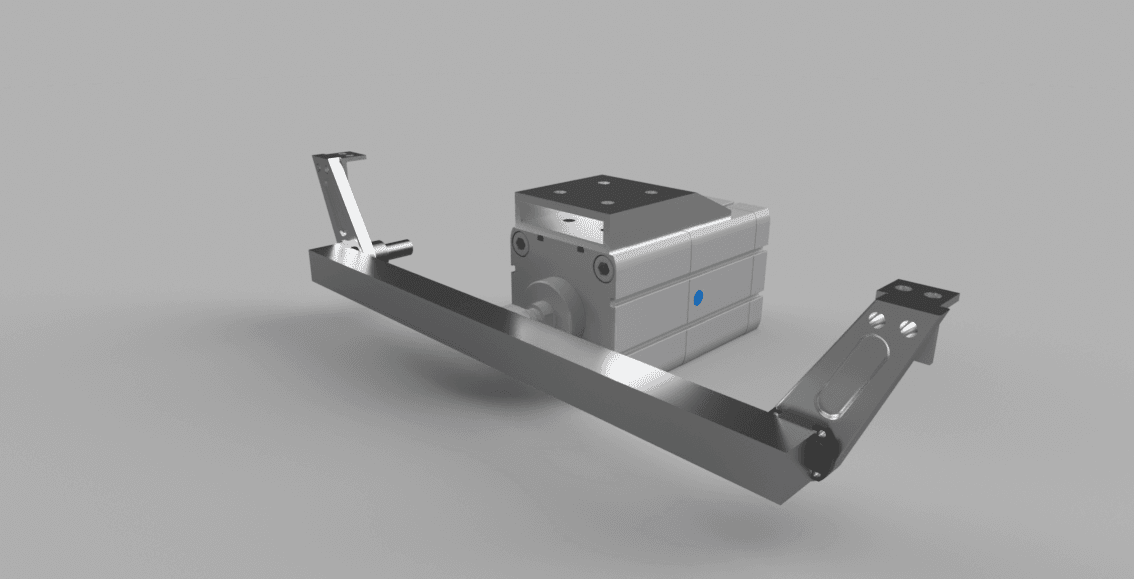
\includegraphics[width =\linewidth]{images/EC_Brake_Master_2018}
        \label{fig:EC-Assembly}
        \caption{The Master Assembly of the EC Brakes}
    \end{figure}
    
    \begin{figure}
    	\centering
        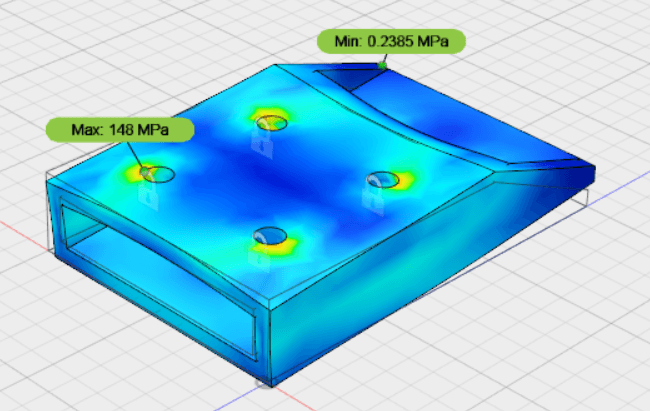
\includegraphics[width =\linewidth]{images/ECPistonMount}
        \label{fig:ECPiston}
        \caption{FEA of the Piston mount for the Eddy Current Brakes}
    \end{figure}
    
    \begin{figure}
    	\centering
        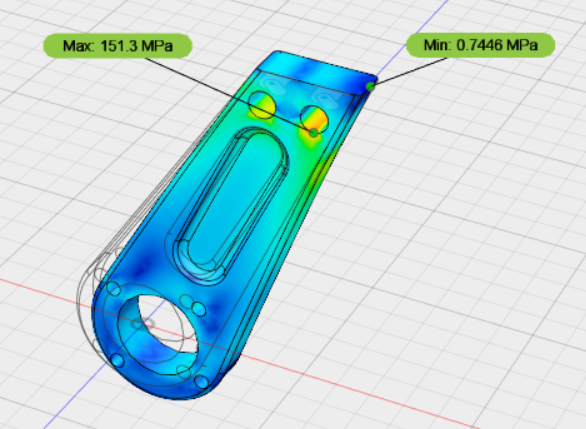
\includegraphics[width = \linewidth]{images/ShaftMount}
        \label{fig:ShafttMount}
        \caption{FEA of the Shaft Mount for the Eddy Current Brakes}
    \end{figure}
    
    \begin{figure}
    	\centering
        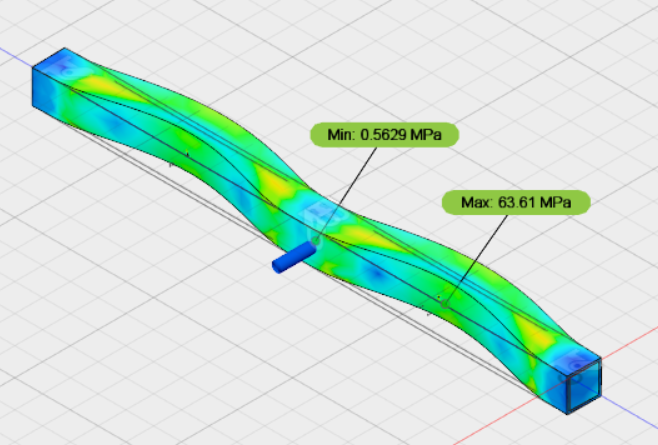
\includegraphics[width=\linewidth]{images/MagnetBarFEA}
        \label{fig:MagnetBar}
        \caption{FEA of the Magnet Bar}
    \end{figure}

     \begin{figure}
        \centering
        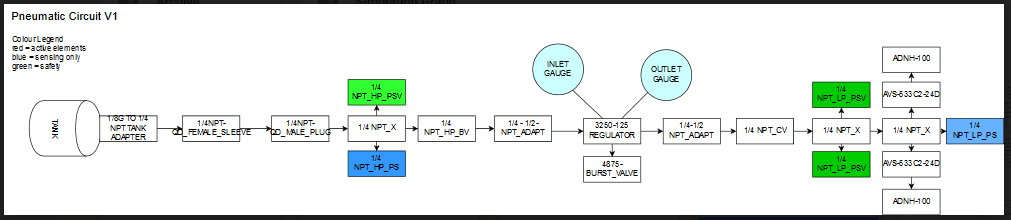
\includegraphics[width=\linewidth]{images/EC_Pnuematic_Circuit.png}
        \caption{The pneumatic circuit that we will be using to power the actuators of the brakes}
        \label{fig:pneumatic-circuit}
    \end{figure}
    
    [Comments on how this integrates with friction braking calipers]\\
    Full labeled detailed CAD\\
    Mass, power, etc.\\
    How is it failsafe?\\
    Full cost breakdown, comments on manufacturability and production costs\\
    “A full Bill of Materials can be found in Appendix C.”

    \subsection{Physical Modeling}
    \begin{table}
    	\centering
    	\begin{tabular}{ll} \toprule
            Parameters & Value\\ \midrule
            Dimensions(\si{m})     & 0.0254 $\times$ 0.0254 $\times$ 0.0254 \\
            Material     & NdFeB, Grade N52   \\
            Pull Force(\si{N})     & 165.34 \\
            Operating Temperature     & 353K  \\ \bottomrule
        \end{tabular}
        \caption{Magnet Specifications}
        \label{table:magnets}
    \end{table}
    Our Eddy current brakes will be made with 2 arrays of 16 magnets (see \reftab{table:magnets} for magnet specifications) on either side of the rail. The array of magnets will be made using Halbach arrays, as seen in \reffig{fig:halbach-array}, which is a way of arranging magnets that increase the magnetic flux on one side of the array.\\

    \begin{figure}
        \centering
        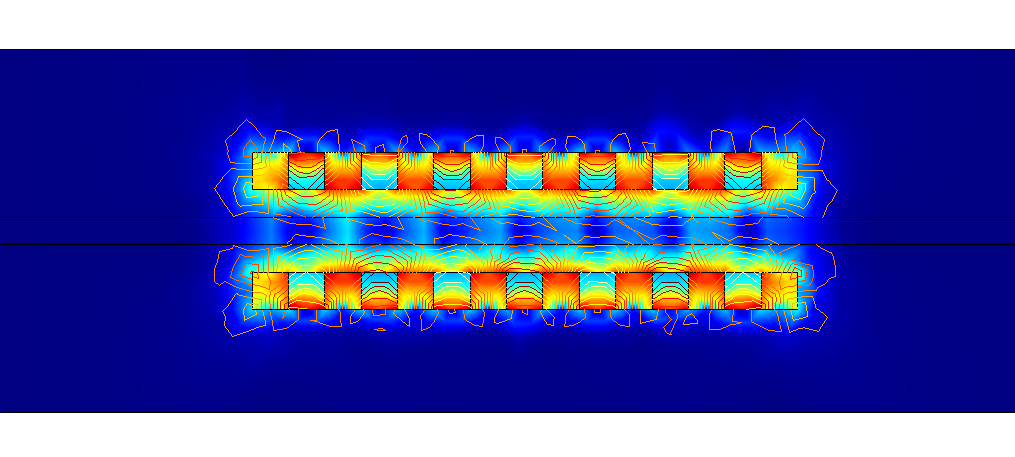
\includegraphics[width=\linewidth]{images/halbach_array.png}
        \caption{Halbach Array on the Rail}
        \label{fig:halbach-array}
    \end{figure}
     Since we are using magnets for the brakes there will be a force created. Both perpendicular and parallel to the actual rail. The equation for the lift force, which in this case is the force perpendicular to the rail.
     \begin{equation}\label{eq:lift-force}
     F_{\textrm{Lift}} = \frac{3\mu m^2}{32\pi z_0^4}\times\left(1 -\frac{\omega}{\sqrt[2]{v^2+\omega^2}}\right)
    \end{equation}
    Where $\mu$ is the vacuum permeability, m is the magnetic vertical dipole moment, $\omega$ is the velocity of magnetic propagation through the beam and $z_0$ is the separation of the magnets from the rail. While the magnitude of the drag force that will be created is given by
    \begin{equation}\label{eq:lift-force2}
    \left\lvert F_{drag}\right\rvert = \frac{\omega}{v} F_{lift}
    \end{equation}
     Using Equations \ref{eq:lift-force} and \ref{eq:lift-force2} we were able to graph the forces that we would expect from speeds between 0-\SI{100}{m/s} where $z_0 = \SI{18}{mm}$.\\

    \begin{figure}
        \centering
        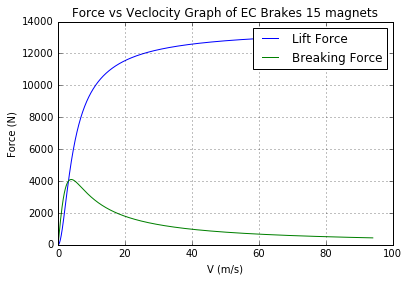
\includegraphics[width=\linewidth]{images/force_velocity_graph.png}
        \caption{Graph of the lift and drag forces experienced by the magnets, for one of the brakes}
        \label{fig:force-velocity-graph}
    \end{figure}
    Based on the graphs for force and velocity in \reffig{fig:force-velocity-graph}, we were able to determine the velocity profile (\reffig{fig:velocity-profile}), acceleration profile (\reffig{fig:accelation-profile}), and the distance profile (\reffig{fig:distance-profile}).\\

 	\begin{figure}
        \centering
        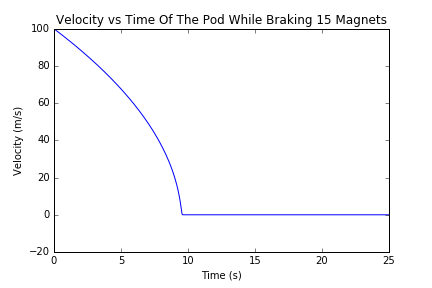
\includegraphics[width=\linewidth]{images/velocity_time_graph}
        \caption{Velocity Profile During Braking}
        \label{fig:velocity-profile}
    \end{figure}
    \begin{figure}
        \centering
        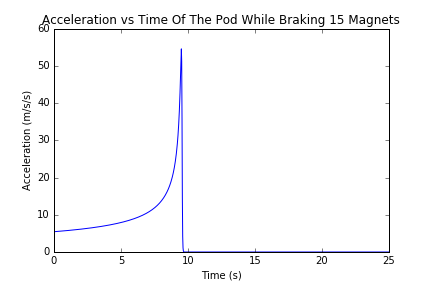
\includegraphics[width=\linewidth]{images/acceleration_time_graph}
        \caption{Acceleration Profile During Braking}
        \label{fig:accelation-profile}
    \end{figure} 
    \begin{figure}
        \centering
        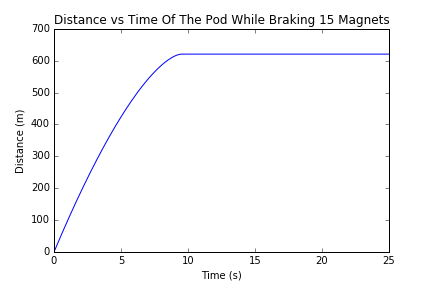
\includegraphics[width=\linewidth]{images/distance_time_graph}
        \caption{the distance traveled in during braking}
        \label{fig:distance-profile}
    \end{figure}
    
    From the force graphs it becomes evident that the pod will have to endure large forces when breaking. We can expect a maximum lift force of around 14000N and a maximum drag force of around \SI{4000}{N}. This means that the mounting to the frame and the position of the actuator need to be able to withstand these forces. The mounting points on the frame have been designed to be able to handle this force. The actuator is going to be oriented perpendicular to the magnets. Initially we thought about angling the actuator, this way the actuator would only experience some of the total force and not at its entirety. It was decided against this idea because this would require that we use an actuator with a larger stroke length. This would create a large bending moment which would not be ideal. As well the larger stroke length leads to the another problem of a large bending moment.
    From the acceleration time graph we can also see that at slower speeds, there is a spike in the drag force. This would create an acceleration of around 6Gs, which the pod is not designed to handle. Our pod has been designed to be able to safely handle 3Gs. To solve this problem we are going to be using our actuator to slowly retract the brakes at 10m/s at which point the low speed friction brakes would take over and slow the pod down to a complete stop. 
   Taking that into account as well as the expected propulsion we now have a complete idea of what our displacement, velocity and acceleration profiles will look like.
   
    \begin{figure}
        \centering
        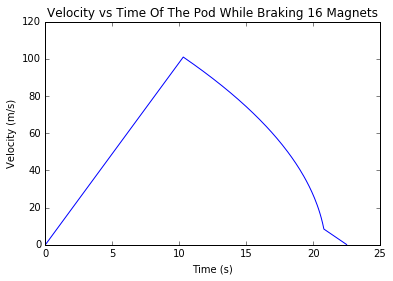
\includegraphics[width=\linewidth]{images/totalvelocityprofile}
        \caption{Velocity Profile for the entire journey of the pod}
        \label{fig:total-velocity-profile}
    \end{figure}
    \begin{figure}
        \centering
        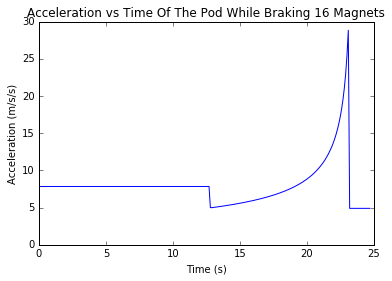
\includegraphics[width=\linewidth]{images/totalaccelerationprofile}
        \caption{Acceleration Profile During Braking}
        \label{fig:total-accelation-profile}
    \end{figure} 
    \begin{figure}
        \centering
        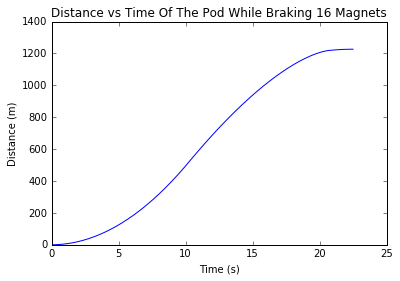
\includegraphics[width=\linewidth]{images/totaldistanceprofile}
        \caption{the distance traveled in during braking}
        \label{fig:distance-profile}
    \end{figure}
    
    Since we are using magnets, that means that there will always be a force related at some separation from the track. That means that when the brakes are in an off state they need to be far enough from the track such that the force that they pod feels is minimal. In order to figure this out what we used the equation for drag force (\ref{eq:lift-force2}) and inputted separation values and determined the one that would give us the lowest maximum drag force that fit our design requirements. From that we found that the optimal distance was 0.049mm away from the track.    
    
 
    \subsection{Thermal}
    One thing that we have to be careful of is the heating that the breaks would have. As stated in the table above the max operating temperature for the magnets is $80$C\textdegree this means that we need to make sure that that the brakes do not get to that level.\\

    \begin{figure}
    	\centering
        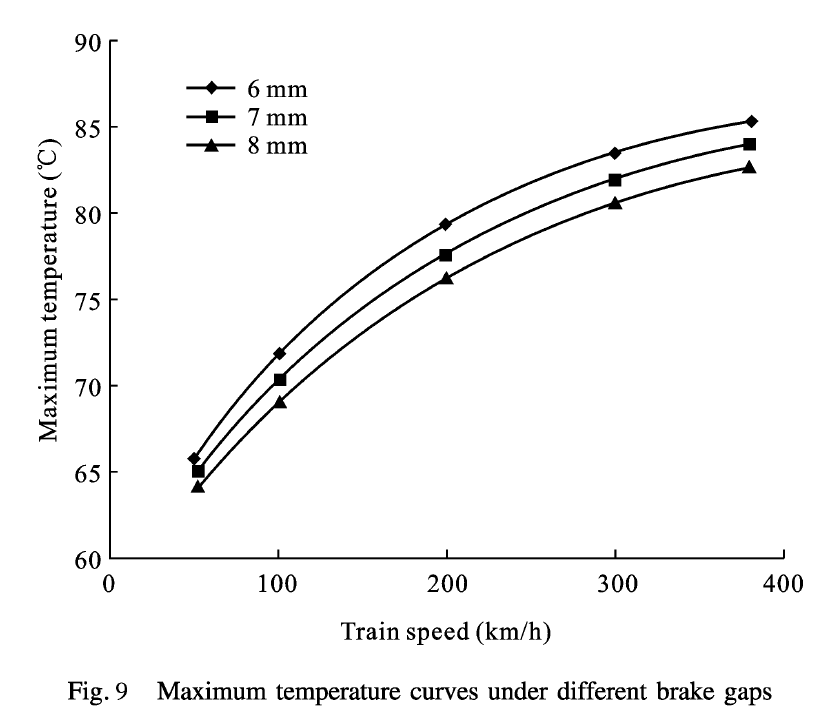
\includegraphics[width=\linewidth]{images/EC_heat}
        \caption{Maximum temperature curves under different brake gaps}
        \label{fig:ec-heat}
    \end{figure}
    \reffig{fig:ec-heat} shows how hot the rail would get at high speeds due to the Eddy Current brakes. For this plot we use a $z_0$ values of 6-\SI{8}{mm}. You can see that at \SI{100}{m/s}, which is the max speed our pod is designed for, the total heating on the rail ranges between 69-\SI{73}{\celsius} from this if we then extrapolate to the value of $z_0 = \SI{19}{mm}$ that we are using we see that the thermal heating due to the Eddy Current brakes will not damage the rail or the magnets in the brakes at all.

    \subsection{Structural}
    One thing that we have to understand of is how these brake will react in the case of failure, electrical or otherwise. For the brakes they require to power to activate, therefore in case of power failure in our main battery we have a backup battery specifically for the brakes that will activate and slow the pod down.  \\
    What are several reasonable and edge-case loading scenarios, and how does the FEA look for all of those? Justify your “reasonable” scenarios. If possible to simulate, how many cycles might it withstand?\\
    How will we deal with imperfections and irregularities in the track, both lateral and vertical? (Simulation would be good)

    \subsection{Tests \& Validation (completed and planned)}
    Test rig (see Next Steps as well)\\
    Fault tolerance, potential failure modes (FMEA)

    \subsection{Safety and handling}
    Neodymium magnets have the ability to damage both equipment and handlers. Therefore, only members of the team that have taken the magnet handling safety course are permitted access to the magnets. When transferring the magnets always hold two separate magnets in opposite hands away from any ferromagnetic metal. Eye protection must be worn when handling the magnets as magnet dust may get into eyes and gloves are recommended. In case of emergency evacuation, place magnets in a safe area away from ferromagnetic metals. 
    
\end{document}
